\documentclass[12pt]{report}
\usepackage[utf8]{inputenc}
\usepackage[russian]{babel}
%\usepackage[14pt]{extsizes}
\usepackage{listings}
\usepackage{graphicx}
\usepackage{amsmath,amsfonts,amssymb,amsthm,mathtools} 
\usepackage{pgfplots}
\usepackage{filecontents}
\usepackage{float}
\usepackage{comment}
\usepackage{indentfirst}
\usepackage{eucal}
\usepackage{enumitem}
%s\documentclass[openany]{book}
\frenchspacing

\usepackage{array}

\usepackage{verbatim}

\usepackage{caption}
\captionsetup{labelsep=endash}
\captionsetup[figure]{name={Рисунок}}

\usepackage{indentfirst} % Красная строка

\usetikzlibrary{datavisualization}
\usetikzlibrary{datavisualization.formats.functions}

\usepackage{amsmath}


% Для листинга кода:
\lstset{ %
	language=c,                 % выбор языка для подсветки (здесь это С)
	basicstyle=\small\sffamily, % размер и начертание шрифта для подсветки кода
	numbers=left,               % где поставить нумерацию строк (слева\справа)
	numberstyle=\tiny,           % размер шрифта для номеров строк
	stepnumber=1,                   % размер шага между двумя номерами строк
	numbersep=5pt,                % как далеко отстоят номера строк от подсвечиваемого кода
	showspaces=false,            % показывать или нет пробелы специальными отступами
	showstringspaces=false,      % показывать или нет пробелы в строках
	showtabs=false,             % показывать или нет табуляцию в строках
	frame=single,              % рисовать рамку вокруг кода
	tabsize=2,                 % размер табуляции по умолчанию равен 2 пробелам
	captionpos=t,              % позиция заголовка вверху [t] или внизу [b] 
	breaklines=true,           % автоматически переносить строки (да\нет)
	breakatwhitespace=false, % переносить строки только если есть пробел
	escapeinside={\#*}{*)}   % если нужно добавить комментарии в коде
}


\usepackage[left=2cm,right=2cm, top=2cm,bottom=2cm,bindingoffset=0cm]{geometry}
% Для измененных титулов глав:
\usepackage{titlesec, blindtext, color} % подключаем нужные пакеты
\definecolor{gray75}{gray}{0.75} % определяем цвет
\newcommand{\hsp}{\hspace{20pt}} % длина линии в 20pt
% titleformat определяет стиль
\titleformat{\chapter}[hang]{\Huge\bfseries}{\thechapter\hsp\textcolor{gray75}{|}\hsp}{0pt}{\Huge\bfseries}


% plot
\usepackage{pgfplots}
\usepackage{filecontents}
\usetikzlibrary{datavisualization}
\usetikzlibrary{datavisualization.formats.functions}

\begin{document}
	%\def\chaptername{} % убирает "Глава"
	\thispagestyle{empty}
	\begin{titlepage}
		\noindent \begin{minipage}{0.15\textwidth}
			
\includegraphics[width=\linewidth]{inc/b_logo}
		\end{minipage}
		\noindent\begin{minipage}{0.9\textwidth}\centering
			\textbf{Министерство науки и высшего образования Российской Федерации}\\
			\textbf{Федеральное государственное бюджетное образовательное учреждение высшего образования}\\
			\textbf{~~~«Московский государственный технический университет имени Н.Э.~Баумана}\\
			\textbf{(национальный исследовательский университет)»}\\
			\textbf{(МГТУ им. Н.Э.~Баумана)}
		\end{minipage}
		
		\noindent\rule{18cm}{3pt}
		\newline\newline
		\noindent ФАКУЛЬТЕТ $\underline{\text{«Информатика и системы управления»}}$ \newline\newline
		\noindent КАФЕДРА $\underline{\text{«Программное обеспечение ЭВМ и информационные технологии»}}$\newline\newline\newline\newline\newline
		
		\begin{center}
			\noindent\begin{minipage}{1.1\textwidth}\centering
				\Large\textbf{Отчет по лабораторной работе №7}\newline
				\textbf{по дисциплине <<Моделирование>>}\newline\newline
			\end{minipage}
		\end{center}
		
		\noindent\textbf{Тема} $\underline{\text{Моделирование системы на GPSS}}$\newline\newline
		\noindent\textbf{Студент} $\underline{\text{Слепокурова М.Ф.}}$\newline\newline
		\noindent\textbf{Группа} $\underline{\text{ИУ7-76Б}}$\newline\newline
		\noindent\textbf{Оценка (баллы)} $\underline{\text{~~~~~~~~~~~~~~~~~}}$\newline\newline
		\noindent\textbf{Преподаватель} $\underline{\text{Рудаков И.В.}}$\newline\newline\newline
		
		\begin{center}
			\vfill
			Москва~---~\the\year
			~г.
		\end{center}
	\end{titlepage}

\setcounter{page} {2}


\section*{Постановка задачи}
Промоделировать систему, состоящую из источника информации (ИИ), буферной памяти (БП) и обслуживающего аппарата (ОА), используя среду компьютерного моделирования GPSS World. Источник информации генерирует заявки, время появления которых распределено по равномерному закону, а обслуживающий аппарат обрабатывает каждую из них за время, распределенное по закону Эрланга.
Определить минимальный размер буферной памяти, при котором не будет потерь заявок. Учесть возможность задания вероятности повторного попадания заявок из обслуживающего аппарата в очередь.


\section*{Теория}
\subsection*{Равномерное распределение}
Равномерное распределение описывает случайную величину, принимающую значения, принадлежащие некоторому промежутку конечной длины, при этом плотность вероятности в этом промежутке всюду постоянна.
\newline

Функция распределения равномерной непрерывной случайной величины имеет следующий вид:
\begin{equation*}
	F(x) = \begin{cases}
		0, & x \leq a \\
		\frac{x-a}{b-a}, & a \leq x \leq b \\
		1, & x > b
	\end{cases}
\end{equation*}

Плотность распределения равномерной непрерывной случайной величины имеет следующий вид:
\begin{equation*}
	f(x) = \begin{cases}
		\frac{1}{b-a}, & a \leq x \leq b \\
		0, & \text{иначе}
	\end{cases}
\end{equation*}

В качестве параметров по умолчанию для равномерного распределения использовались значения $a = 1$ и $b = 10$.

\subsection*{Распределение Эрланга}
Распределение Эрланга описывает непрерывную случайную величину, принимающую неотрицательные значения и представляющую собой сумму $n$ независимых случайных величин, распределенных по одному и тому же экспоненциальному закону с параметром $\lambda$.
\newline

Функция распределения Эрланга непрерывной случайной величины имеет следующий вид:
\begin{equation*}
	F(x) = 1 - e^{-x/\lambda} \sum_{i=0}^{n-1} \frac{(x/\lambda)^i}{i!} 
\end{equation*}

Плотность распределения Эрланга непрерывной случайной величины имеет следующий вид:
\begin{equation*}
	f(x) = \frac{x^{n-1}e^{-x\lambda}\lambda^n}{(n-1)!}
\end{equation*}

В качестве параметров по умолчанию для распределения Эрланга использовались значения $n = 9$ и $\lambda = 0.5$.

\section*{Средства реализации}

По условию задача была реализована на языке GPSS.

\section*{Листинг кода}

\begin{lstlisting}
REENTER_PROBABILITY variable 0.3

UNIFORM_LEFT variable 1
UNIFORM_RIGHT variable 10

ERLANG_RATE variable 0.5
ERLANG_SHAPE variable 9


DATASRC     GENERATE (UNIFORM(1,V$UNIFORM_LEFT,V$UNIFORM_RIGHT))
BUFMEM      QUEUE BUFFER_MEMORY
            SEIZE PROCESSOR
            DEPART BUFFER_MEMORY
PROC        ADVANCE (GAMMA(1,0,V$ERLANG_RATE,V$ERLANG_SHAPE))
            RELEASE PROCESSOR
            TRANSFER V$REENTER_PROBABILITY,FINISH,BUFMEM
FINISH      TERMINATE 1
            START 10000
\end{lstlisting}

\clearpage
\section*{Демонстрация работы программы}
На рисунке \ref{fig:pic1} изображен пример работы программы для 10000 заявок с вероятностью повторного попадания заявки в очередь равной 0. По полученным результатам минимальный размер буферной памяти, при котором не будет потерь заявок, равен 7 ед.

\begin{figure}[h!btp]
	\centering
	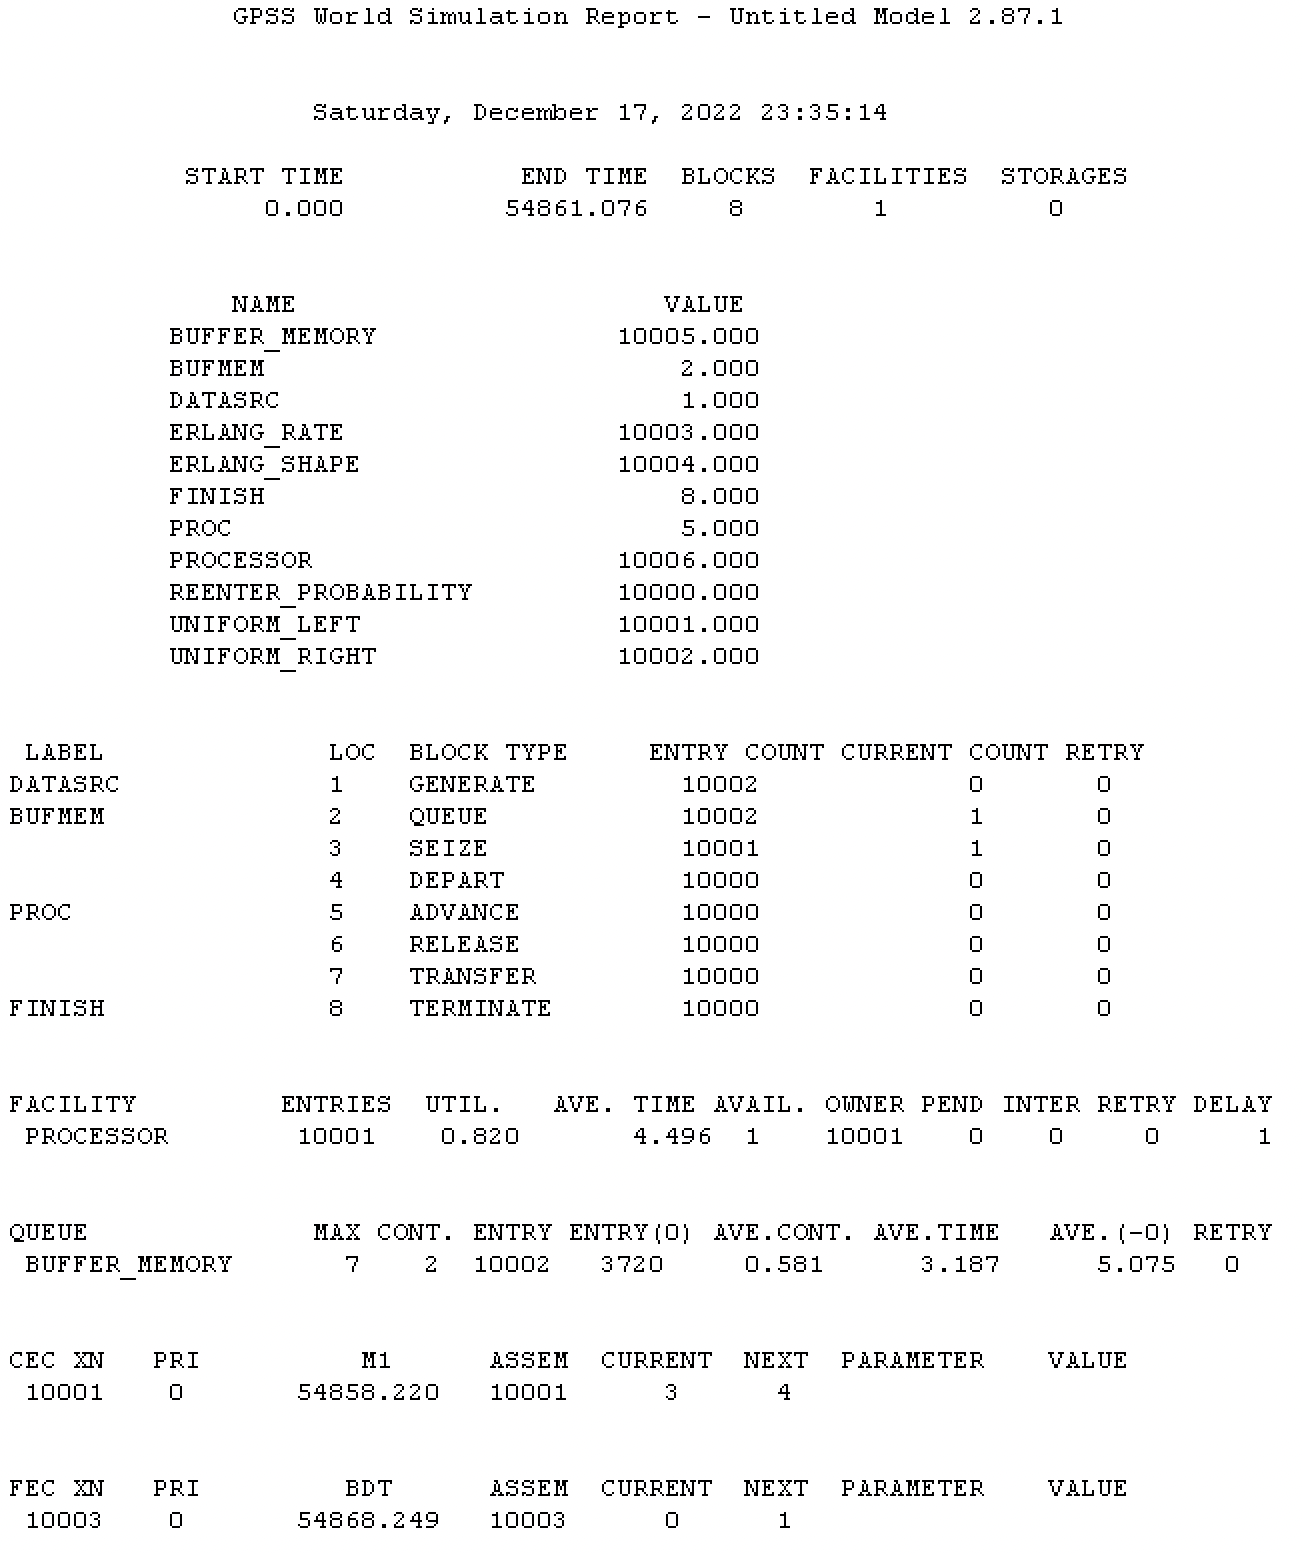
\includegraphics[width=0.8\textwidth]{inc/pic1.png}
	\caption{Пример работы программы --- 1}
	\label{fig:pic1}	
\end{figure}
\clearpage

На рисунке \ref{fig:pic2} изображен пример работы программы для 10000 заявок с вероятностью повторного попадания заявки в очередь равной 0.1. По полученным результатам минимальный размер буферной памяти, при котором не будет потерь заявок, равен 20 ед.

\begin{figure}[h!btp]
	\centering
	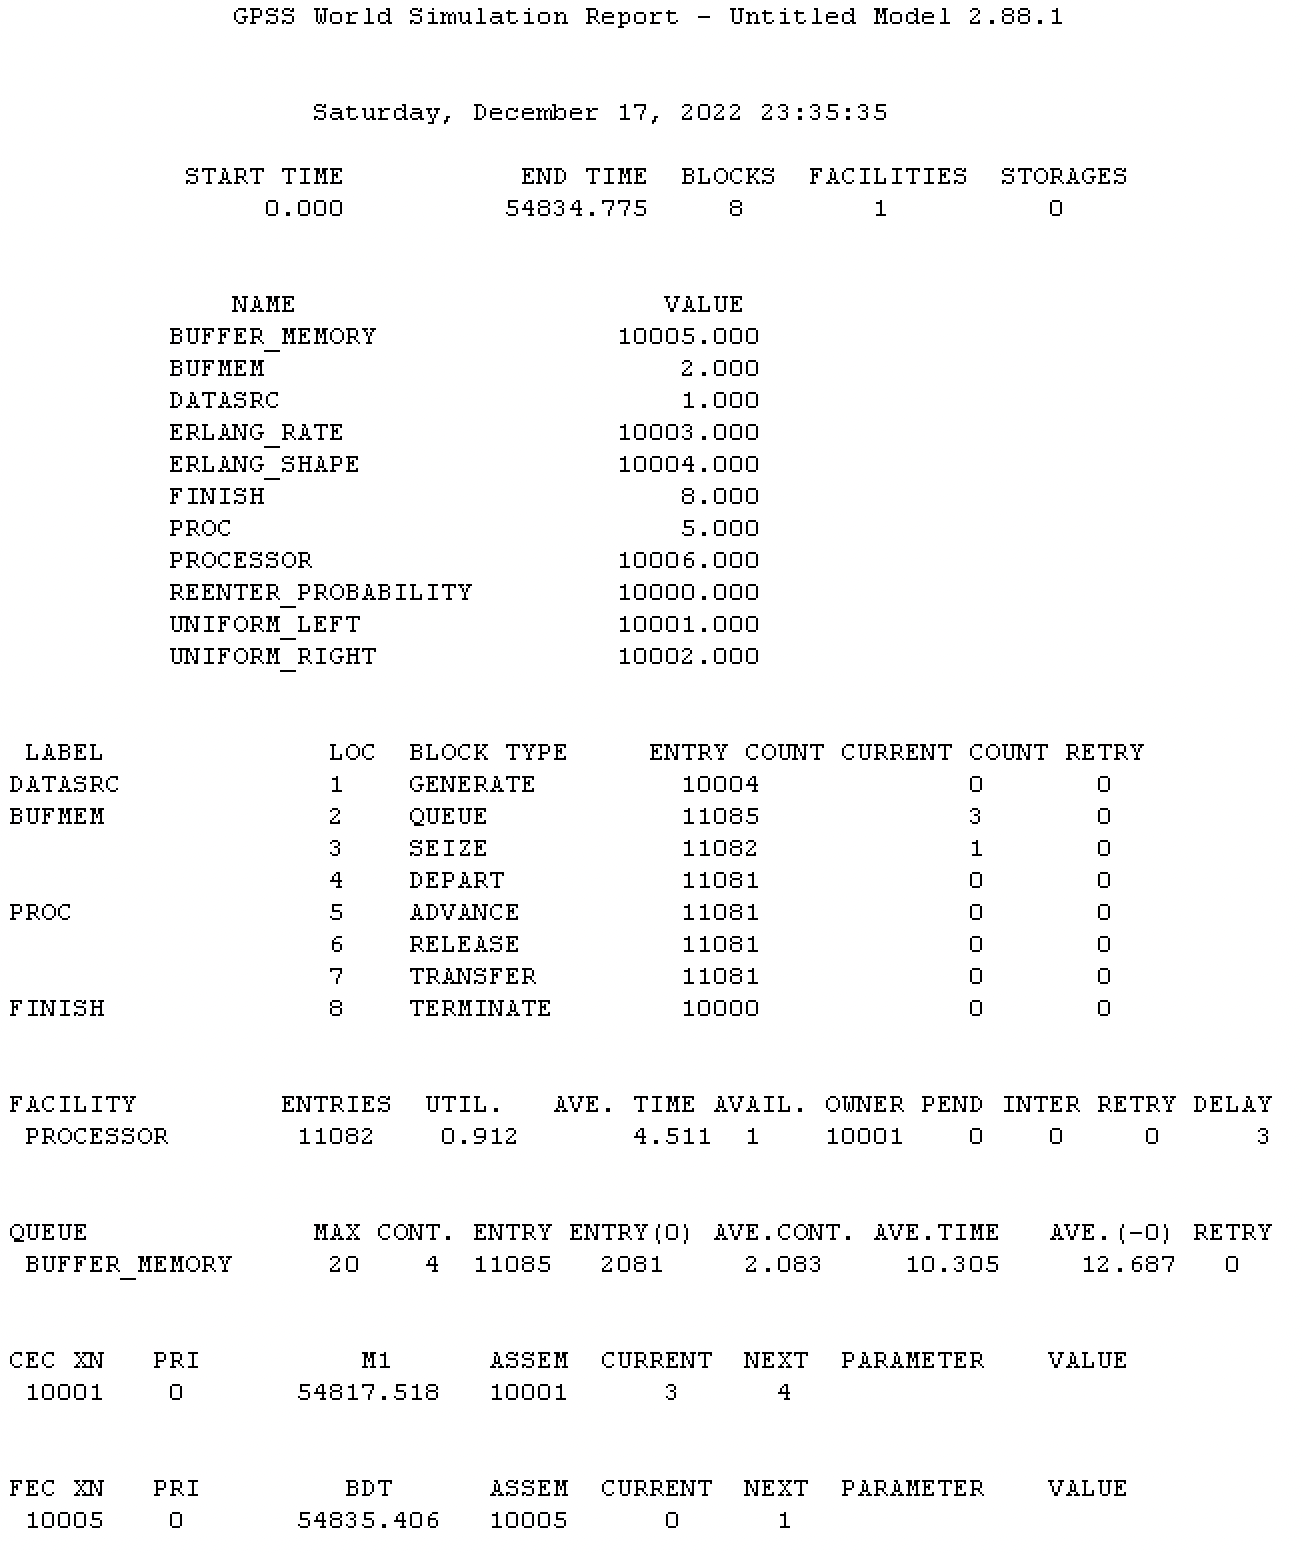
\includegraphics[width=0.8\textwidth]{inc/pic2.png}
	\caption{Пример работы программы --- 2}
	\label{fig:pic2}	
\end{figure}
\clearpage

На рисунке \ref{fig:pic3} изображен пример работы программы для 10000 заявок с вероятностью повторного попадания заявки в очередь равной 0.3. По полученным результатам минимальный размер буферной памяти, при котором не будет потерь заявок, равен 1726 ед.

\begin{figure}[h!btp]
	\centering
	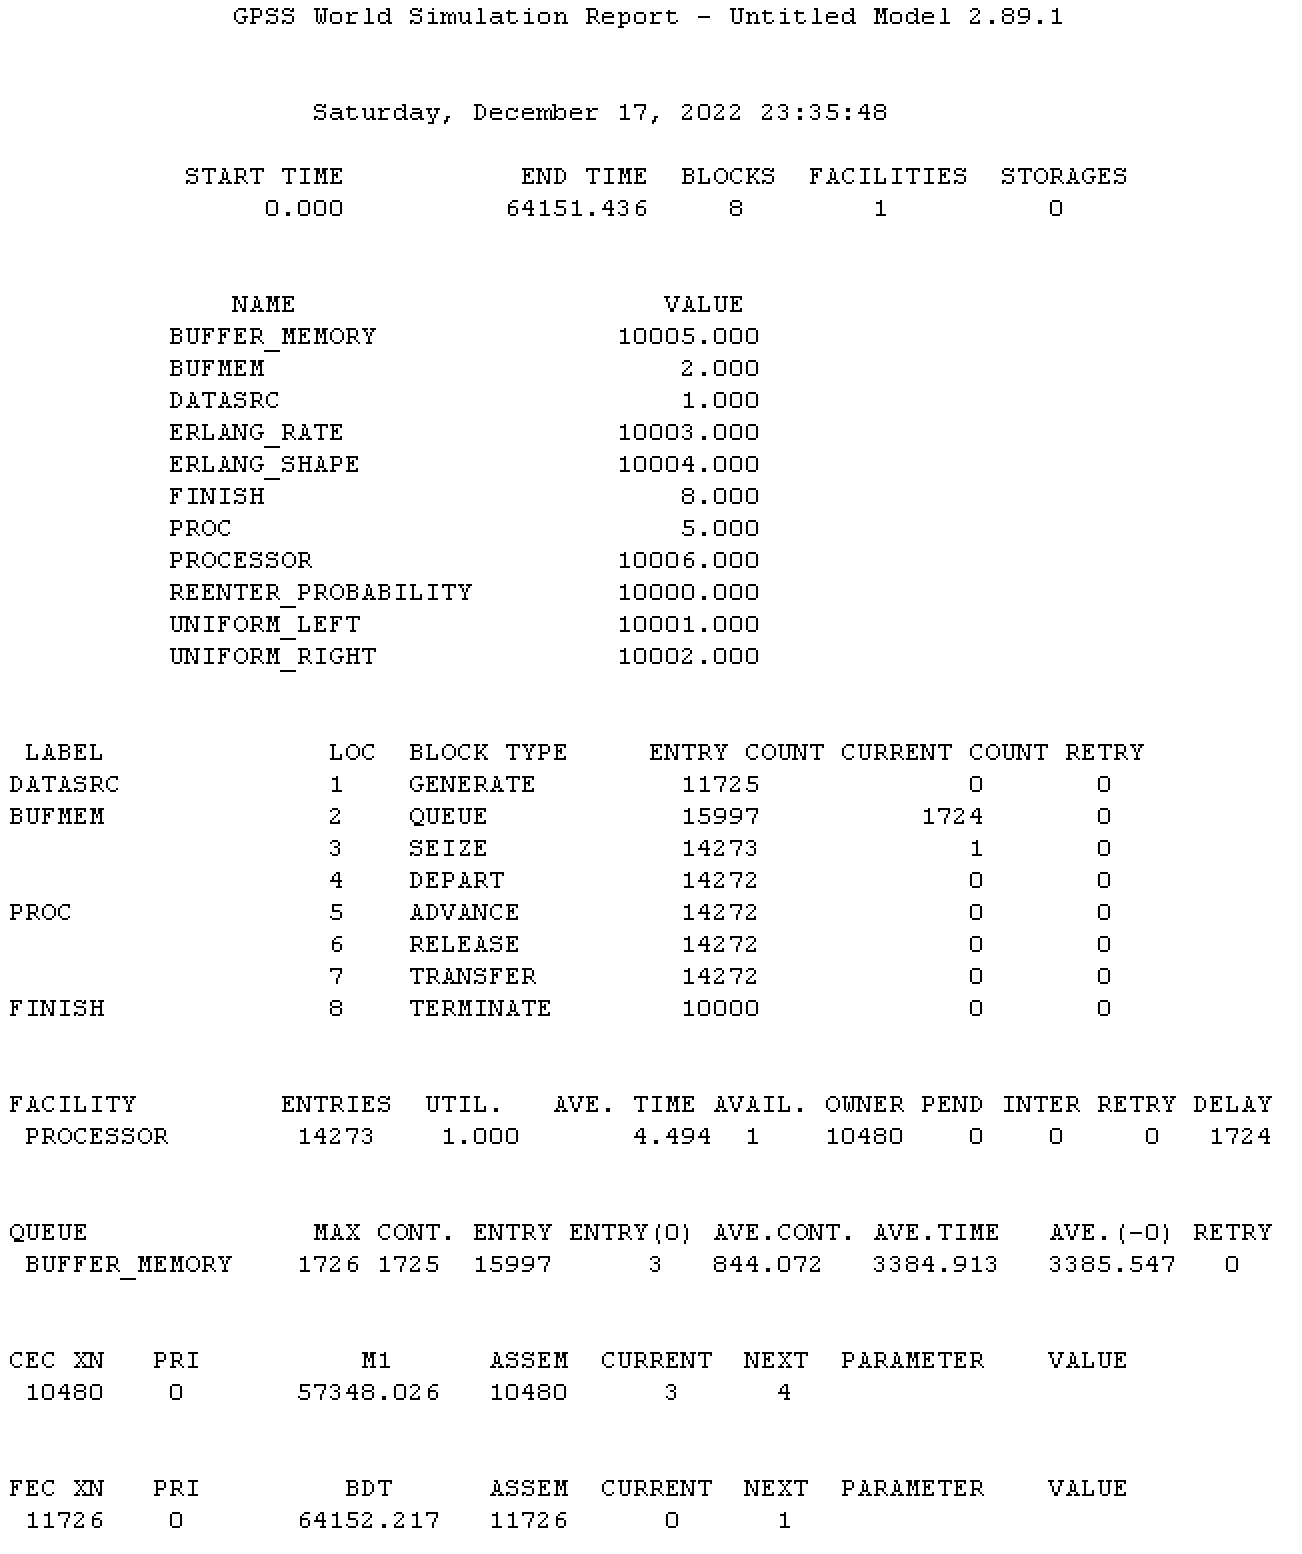
\includegraphics[width=0.8\textwidth]{inc/pic3.png}
	\caption{Пример работы программы --- 3}
	\label{fig:pic3}	
\end{figure}
\clearpage

На рисунке \ref{fig:pic4} изображен пример работы программы для 10000 заявок с вероятностью повторного попадания заявки в очередь равной 0.5. По полученным результатам минимальный размер буферной памяти, при котором не будет потерь заявок, равен 6526 ед.

\begin{figure}[h!btp]
	\centering
	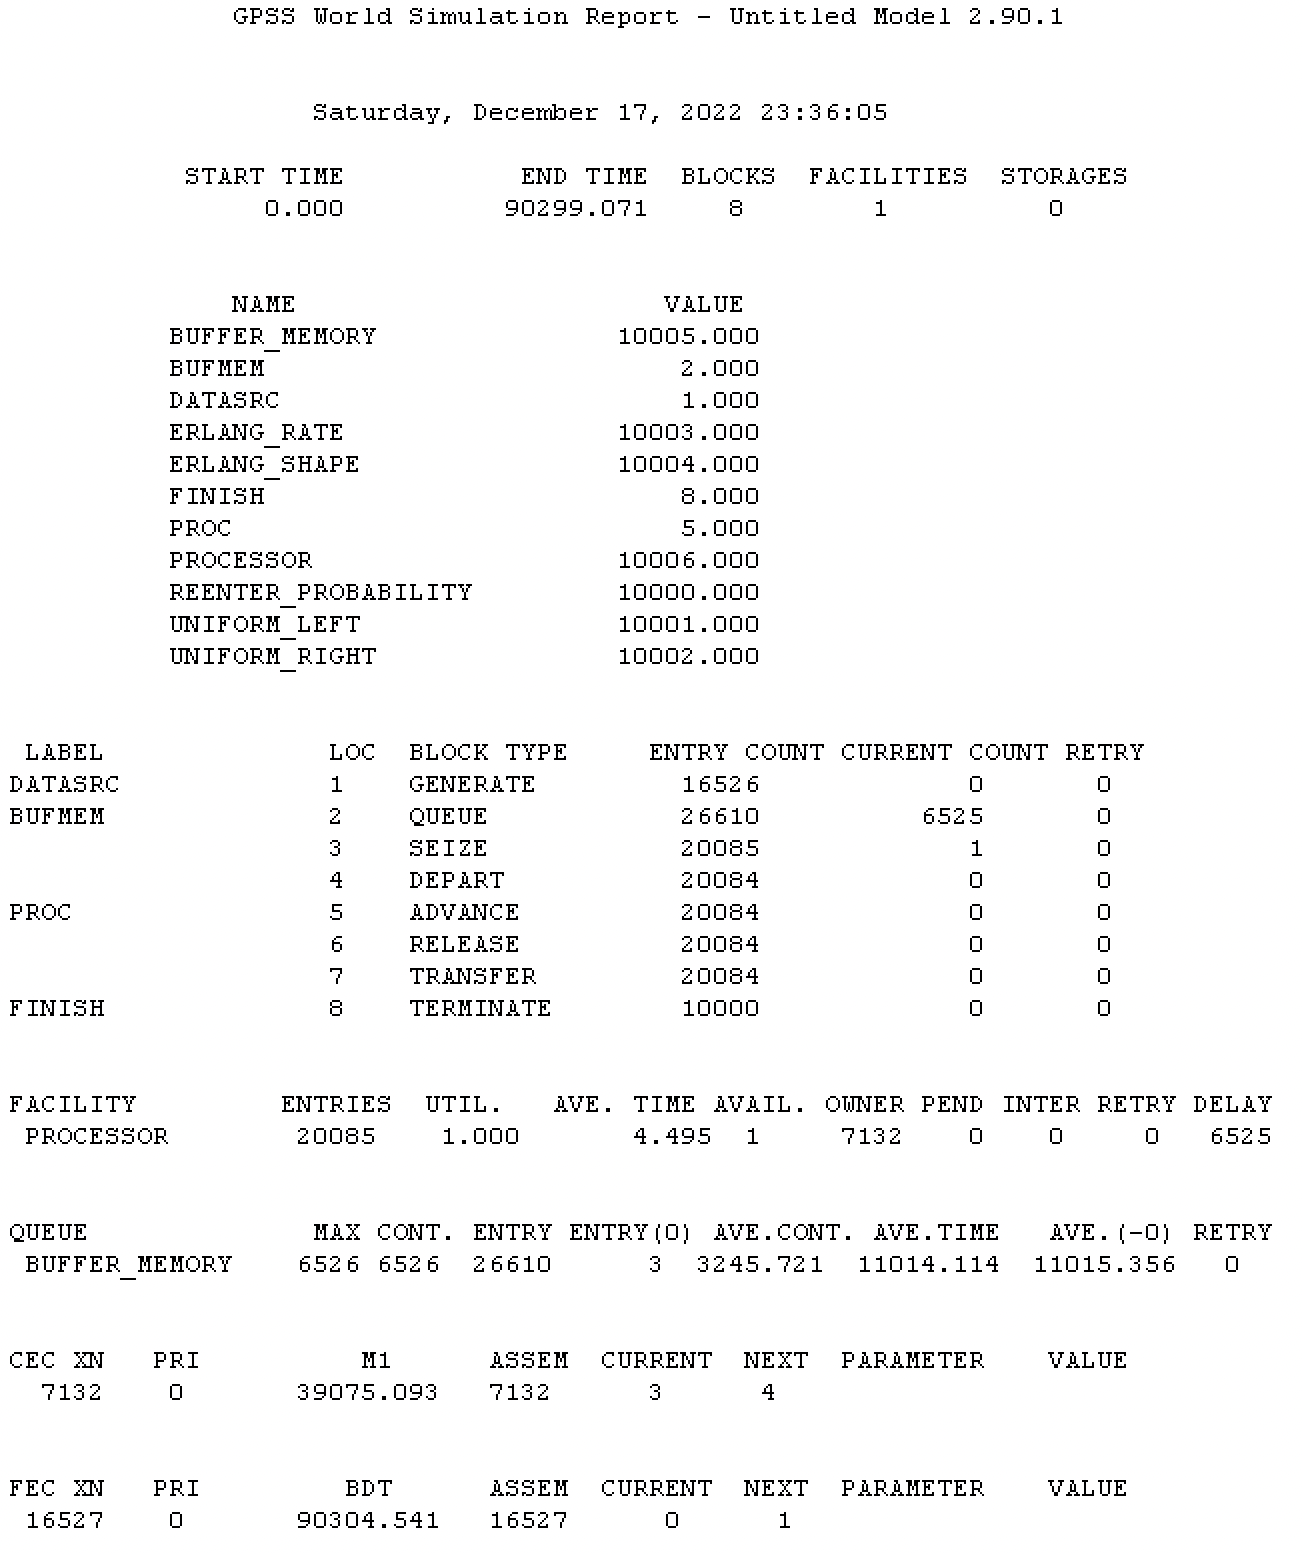
\includegraphics[width=0.8\textwidth]{inc/pic4.png}
	\caption{Пример работы программы --- 4}
	\label{fig:pic4}	
\end{figure}
\clearpage

На рисунке \ref{fig:pic5} изображен пример работы программы для 10000 заявок с вероятностью повторного попадания заявки в очередь равной 0.7. По полученным результатам минимальный размер буферной памяти, при котором не будет потерь заявок, равен 17381 ед.

\begin{figure}[h!btp]
	\centering
	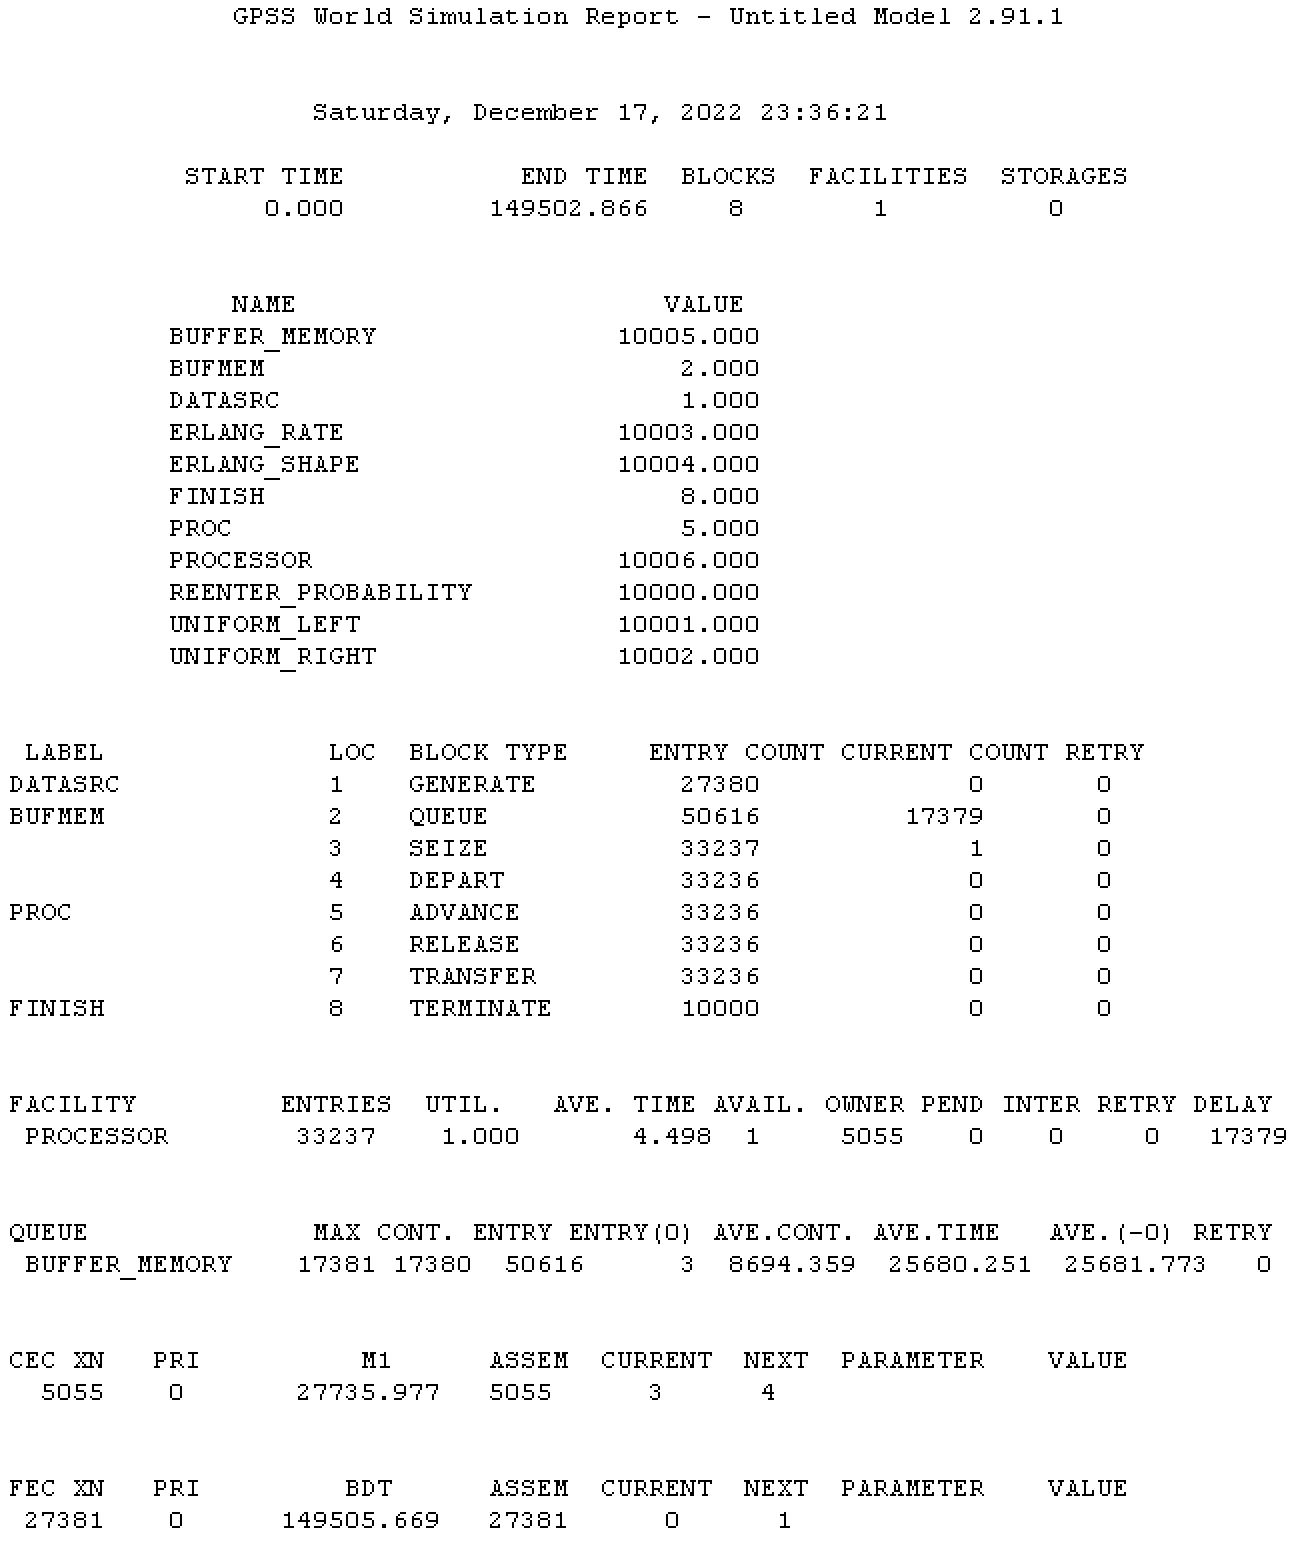
\includegraphics[width=0.8\textwidth]{inc/pic5.png}
	\caption{Пример работы программы --- 5}
	\label{fig:pic5}	
\end{figure}
\clearpage

На рисунке \ref{fig:pic6} изображен пример работы программы для 10000 заявок с вероятностью повторного попадания заявки в очередь равной 0.9. По полученным результатам минимальный размер буферной памяти, при котором не будет потерь заявок, равен 71330 ед.

\begin{figure}[h!btp]
	\centering
	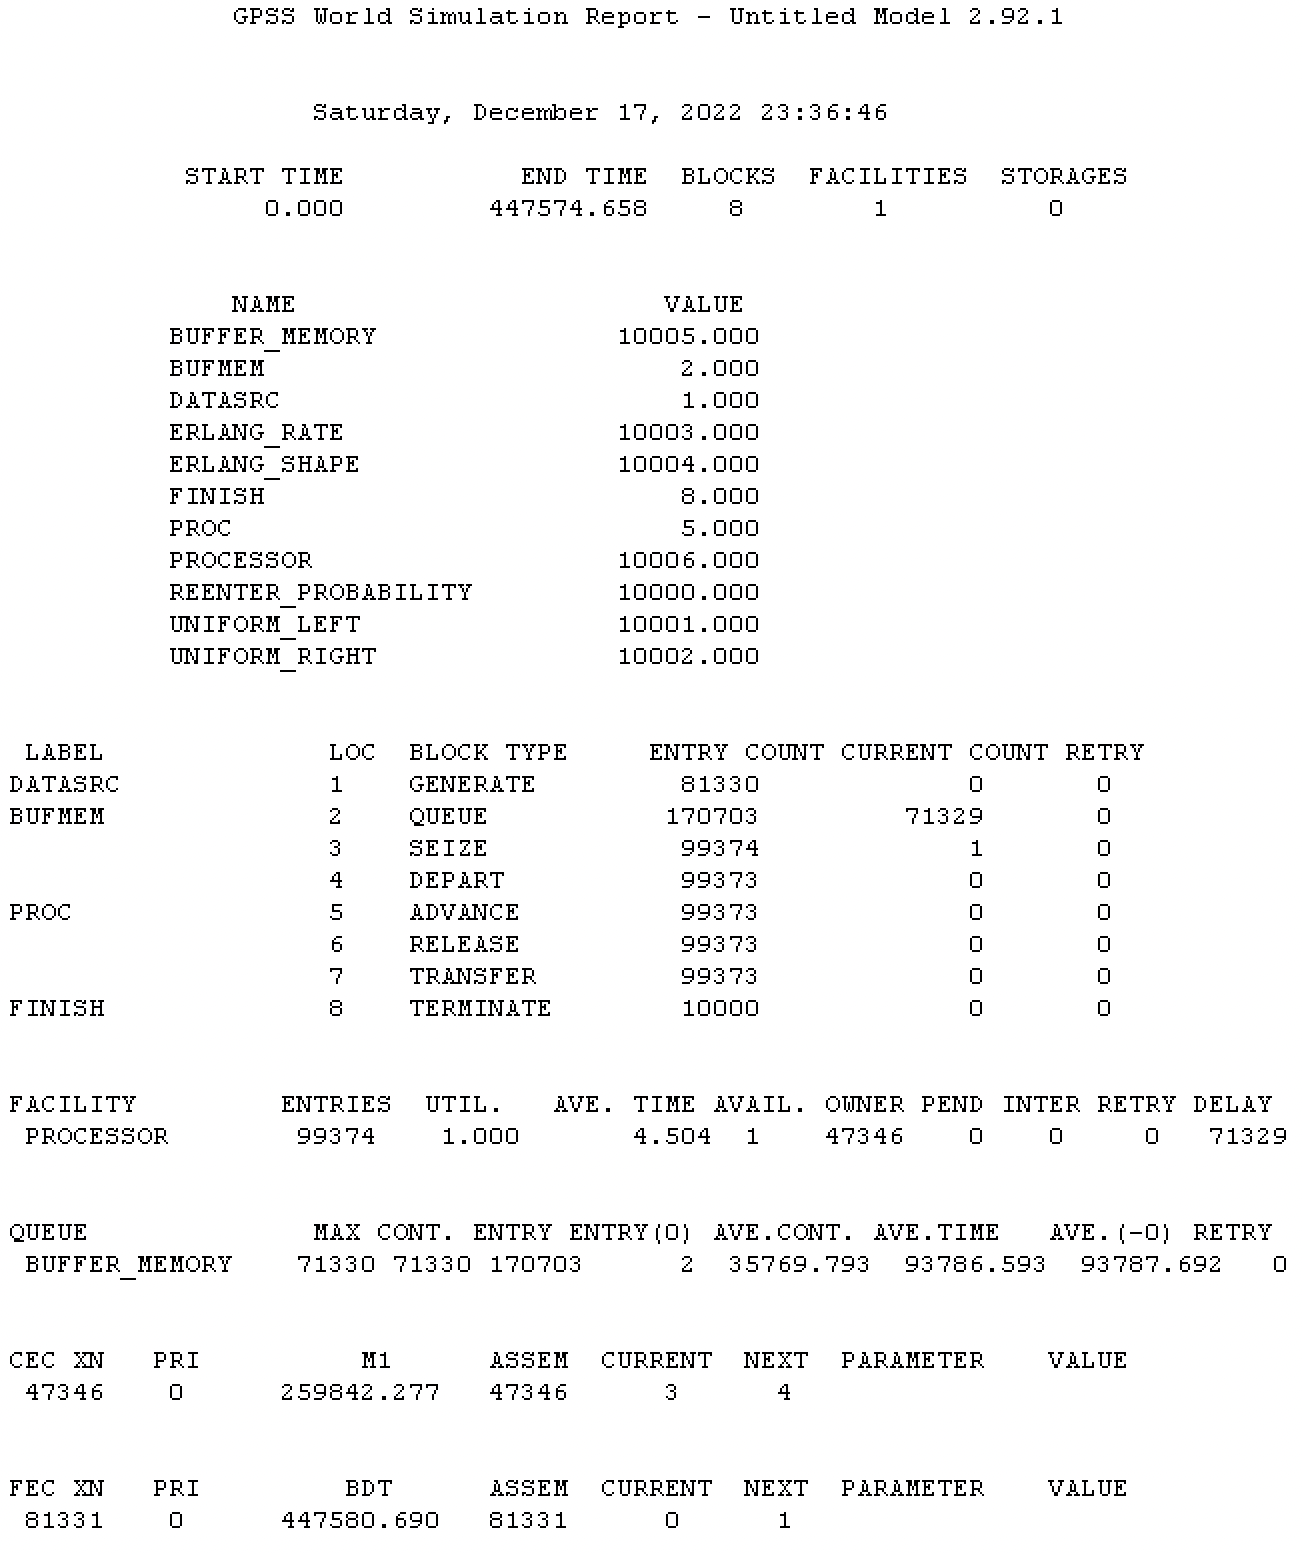
\includegraphics[width=0.8\textwidth]{inc/pic6.png}
	\caption{Пример работы программы --- 6}
	\label{fig:pic6}	
\end{figure}

\bibliographystyle{utf8gost705u}  % стилевой файл для оформления по ГОСТу
\bibliography{51-biblio}          % имя библиографической базы (bib-файла)
	
\end{document}
